\documentclass{article}
\usepackage{graphicx}
\graphicspath{ {images/} }
\usepackage[utf8]{inputenc}
\usepackage{listings}

\title{Programa 2 - Primos}
\author{Leon Tejeda 2CM5}
\date{Octubre 2020}

\begin{document}
\maketitle
\begin{flushleft}
Se nos encargo un programa que encontrara el n-esimo numero primo

INTRODUCCION:

Que es un numero primo:		Es un numero que solo es divisible entre  si mismo y entre la unidad

PLANTEAMIENTO DEL PROBLEMA:

Programar el lenguaje binario definido por los números primos. Dada una "n" que introduzca el usuario o que el programa lo determine automáticamente. El rango de "n" debe de estar en el intervalo de [2,1000000]. "n" determina hasta qué número primo se desea calcular.

1. El programa debe de preguntar si quiere calcular otra "n" o no.

2. La salida, expresada en notación de conjunto, debe ir a un archivo de texto.

3. Del archivo de salida, graficar el número de 1s de cada cadena. El eje de las "x" es la cadena y el eje de las "y" el número de 1s que tiene esa cadena. Específicamente, calcular y graficar cuando n=800000. Al mismo tiempo, calcular la gráfica pero calculando su logaritmo en 
base 2 y 10 respectivamente.

IMPLEMENTACION:

Implementamos un codigo que primero checaba si un numero era primo

Despues se transformaba a  binario y se contaban la cantidad de 1's que este tenia

La cantidad de unos se guardaba junto con el numero de la cadena

Se grafica y = 1's de la cadena  y x = numero de la cadena



Codigo:

\begin{lstlisting}

import random
import os
import math
import cmath
from matplotlib import pyplot

#Coordenadas de la Grafica
def pasar_coordenadas1(x, y):
    archivo = open("Programa2_Coordenadas1.txt", "a")
    archivo.write(str(x))
    archivo.write(",")
    archivo.write(str(y))
    archivo.write("\n")
    archivo.close()
    
    
def grafica(k, limite_y):
     
    archivo = open("Programa2_Coordenadas1.txt", "r")
    for coordenada in archivo:
        x = False
        y = False
        separacion = False
        
        for dato in coordenada:
            if dato != "," and dato !=" " and separacion == False:
                if x == False:
                    x = dato
                
                else:
                    x = x + dato
            
            elif dato != "," and dato !=" " and separacion == True:
                if y == False:
                    y = dato
                
                else:
                    y = y + dato
            else:
                separacion = True
                
        pyplot.plot(int(x), int(y), marker=".", color="blue")
        
        # Logaritmo base 2
        if int(y) != 0:
            y2 = math.log2(int(y))
        else:
            y2=0
            
        pyplot.plot(int(x), y2, marker=".", color="red")

        # Logaritmo base 10
        if int(y) != 0:
            y10 = math.log10(int(y))
        else:
            y10=0
            
        pyplot.plot(int(x), y10, marker=".", color="green")
                
                
    # Establecer el color de los ejes.
    pyplot.axhline(0, color="black")
    pyplot.axvline(0, color="black")
    
    # Limitar los valores de los ejes.
    pyplot.xlim(0, k)
    pyplot.ylim(0, limite_y)
    
    #Salva la Grafica
    pyplot.savefig("Programa2_Grafica1.png")
    
    # Mostrarlo.
    pyplot.show()

            
    archivo.close()

#cuenta cuantos 1s hay en el numero binario
def unos(numero):
    unos = 0
    if numero >= 1:
        while numero > 1:
                
            residuo = numero % 2
            numero = numero // 2
                
            if residuo == 1:
                unos = unos + 1
        
        unos = unos + 1
                            
    return unos

#Transformador (Deccimal-Binario)
def trans_binario(numero):
    binario = 0

    #print ("Transformando a binario....")

    if numero > 1:
        while numero > 1:
                
            residuo = numero % 2
            numero = numero // 2
                
            if binario == 0:
                binario = str(residuo)
                    
            else:
                binario = str(residuo) + binario
        
        binario = str(numero) + binario
                
    else:
        binario = str(numero)
        
    return binario

#Archivo 1 (Forma de Conjunto)
def pasarlo_archivo1(binario, actual, final):
    archivo = open("Programa2_Archivo1.txt", "a")
    if actual == 1:
        archivo.write("{")
        archivo.write(binario)
        archivo.write(",")
        
    elif actual != final:
        archivo.write(binario)
        archivo.write(",")
    
    else:
        archivo.write(binario)
        archivo.write("}")
    archivo.close()

#Checa si es Numero Primo
def es_primo(numero):
    for i in range (2,numero):   
        aux = numero // i
        if aux * i == numero:
            return 0
    return numero

#Programa Central
def primos(n):
    numero = 2
    cantidad = 1
    limite_y = 0
    while cantidad <= n:
        primo = es_primo(numero)
        if primo != 0:
            primo_binario = trans_binario(primo)
            pasarlo_archivo1(primo_binario, cantidad, n)
            coordenada_y = unos(primo)
            pasar_coordenadas1(cantidad, coordenada_y)  
            cantidad = cantidad + 1
            
            if limite_y < coordenada_y:
                limite_y = coordenada_y
        
        numero = numero + 1
        
    grafica(n, limite_y)
            
#Resetea los arhicov y los formatea
def borrar_archivo_existente():
    archivo = open("Programa2_Archivo1.txt", "w")
    archivo.close()
    
    archivo = open("Programa2_Coordenadas1.txt", "w")
    archivo.close()
        

def menu():
    print("Seleccione una opcion")
    print("1. Ingresar un numero entre 2-1000000")
    print("2. Generar un numero aleatorio entre 2-1000000")

    op = int(input(""))

    if op == 1:
        print("Ingrese un numero entre 2-1000000")
        n = int(input(""))
        primos(n)
        
    elif op == 2:
        n = random.randint(2, 1000000)
        print("El numero aleatorio es igual a: " + str(n))
        primos(n)
        
    else:
        print("Ingrese un numero valido")


repetir = 1

while repetir == 1:
    borrar_archivo_existente()
    menu()
    print("Si desea ingresar otro numero presione (y)")
    respuesta = input("")
    os.system("cls")
    
    if respuesta != 'y' and respuesta != 'Y':
        repetir = 0

\end{lstlisting}

FUNCIONAMIENTO:

Adjuntaremos imagenes de cuando n=1000 (incluyendo grafica), ya que con el valor solicitado, no puede graficarse al ser muchas coordenadas

Cuando n = 1000

Menu del programa
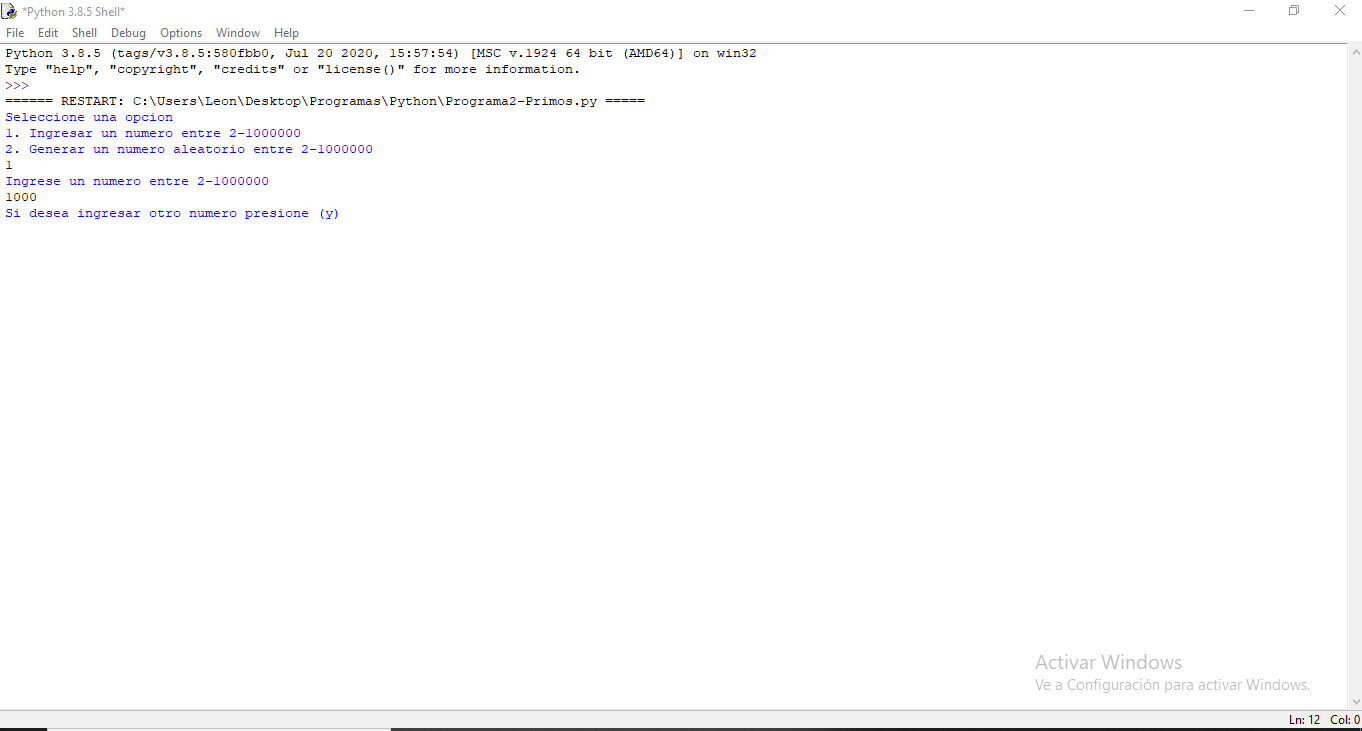
\includegraphics[width= 15cm, height= 5cm]{p2ar1.png}

Esta es la forma en la que imprime los datos en forma de conjuto
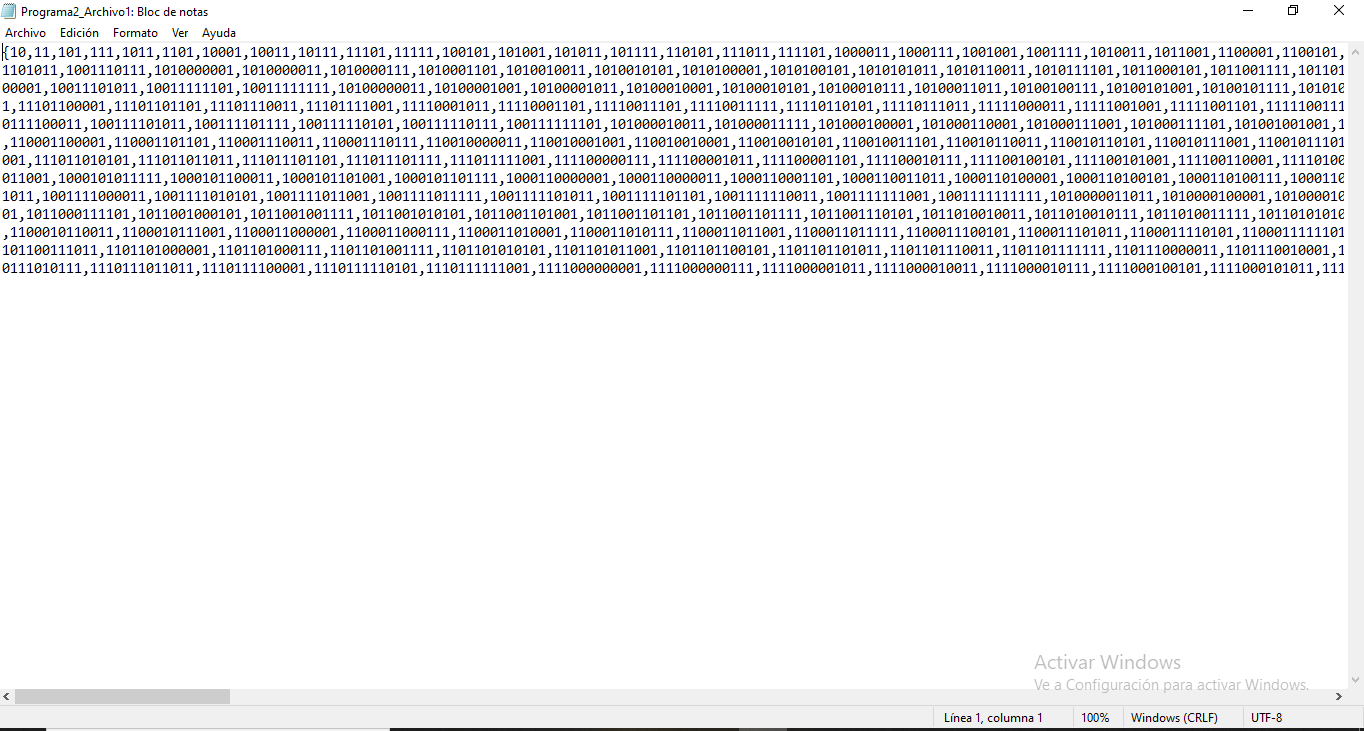
\includegraphics[width= 15cm, height= 5cm]{p2ar2.png}

Coordenadas por cantidad de 1's
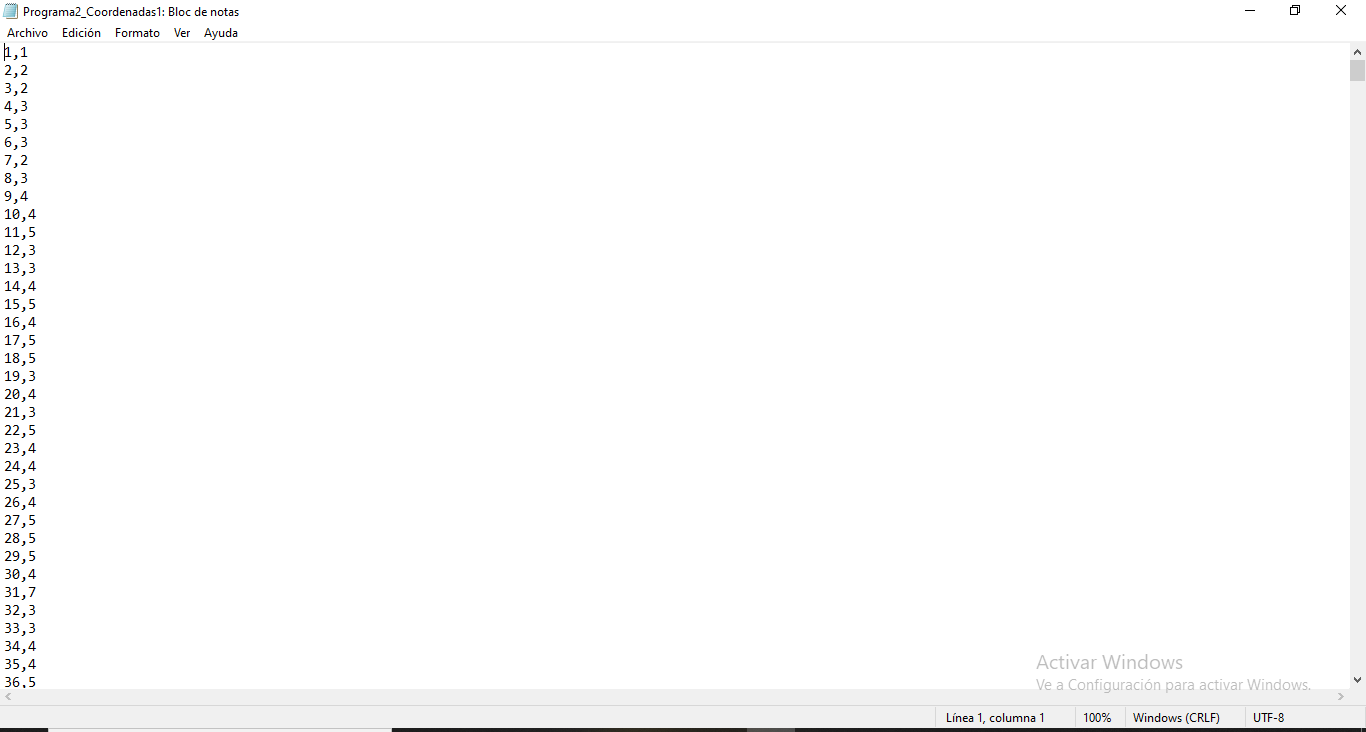
\includegraphics[width= 15cm, height= 5cm]{p2ar3.png}

Grafica por cantidad de 1's

azul = cantodad de 1's
rojo = log2
verde log10
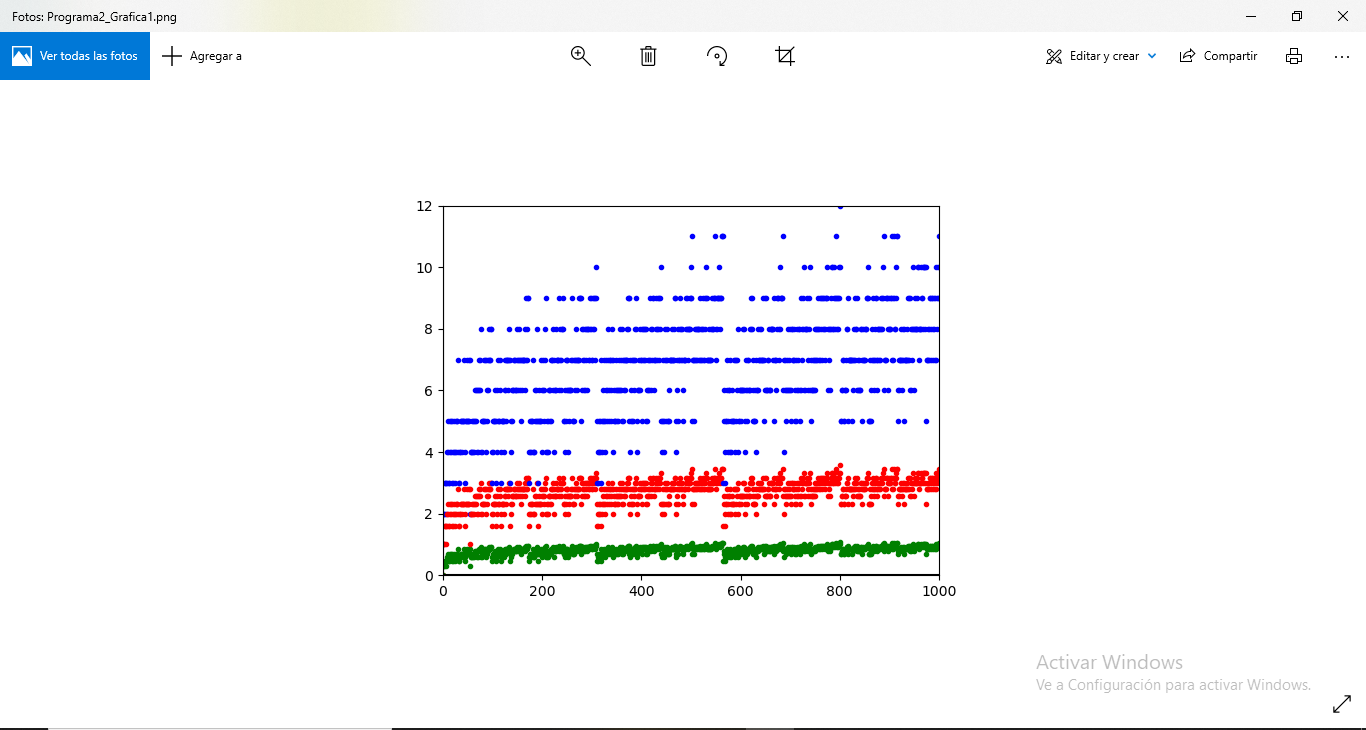
\includegraphics[width= 15cm, height= 5cm]{p2ar4.png}


\end{flushleft}
\end{document}